% gc-termtest-B.tex

\documentclass[11pt]{article}
\usepackage{alltt}
\usepackage{enumerate}
\usepackage{syllogism} 
\usepackage{october}
\usepackage[table]{xcolor}
\pagestyle{empty}

\newcounter{aufg}
\setcounter{aufg}{0}
\newcommand{\aufgabe}[1]{\refstepcounter{aufg}\textbf{(\arabic{aufg})}[#1 points]}

\begin{document}

\textbf{Term Test B version 1}

\aufgabe{5} A conical tent is to have 1000ft$^{3}$ capacity. Find its dimensions if the amount of canvas is to be a minimum. Disregard the floor. Note that the formula for the volume of a cone is
\begin{equation}
\label{eq:uapaighi}
V=\frac{1}{3}r^{2}\pi{}h\notag
\end{equation}
The formula for the area of the lateral surface of a cone (without the floor) is
\begin{equation}
\label{eq:chaekaec}
A=\pi{}rs\notag
\end{equation}
where $s$ is the slant height (see diagram).
\begin{figure}[h]
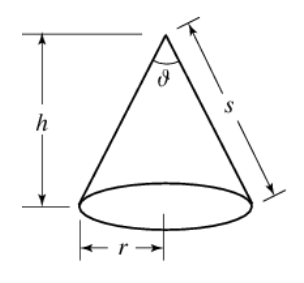
\includegraphics[scale=0.5]{./diagrams/coneslantheight.png}
\end{figure}

\aufgabe{5} Evaluate the following limit.
\begin{equation}
\label{eq:ahkisoav}
\lim_{x\rightarrow\frac{pi}{4}}\frac{\sin{}x-\cos{}x}{x-\frac{\pi}{4}}\notag
\end{equation}

\aufgabe{5} Differentiate
\begin{equation}
\label{eq:aphaefex}
g(t)=neft(\sinheft(2t
ight)
ight)
\end{equation}

\aufgabe{5} An open-top box is to be made by cutting small congruent squares from the corners of a 13 inch by 13 inch sheet of tin and bending up the sides. How large should the squares cut from the corners be to make the box hold as much as possible?
\begin{figure}[h]
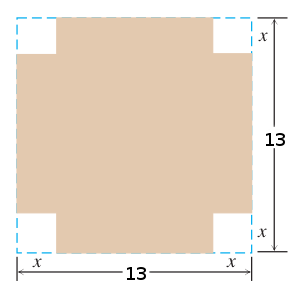
\includegraphics[scale=0.5]{./diagrams/gc-termtestB-v1-01.png}
\end{figure}

\aufgabe{5} Evaluate the following limit.
\begin{equation}
\label{eq:voolohqu}
\lim_{x\rightarrow\frac{\pi}{2}}\frac{2x-\pi}{\cos{}x}\notag
\end{equation}

\aufgabe{5} Analyze the following function (do not worry about asymptotes and whether the function is even/odd). This means that you need to find the following:
\begin{itemize}
\item domain and range
\item $x$-intercepts
\item critical points (indicate if they are maxima or minima)
\item inflection points
\end{itemize}
\begin{equation}
\label{eq:phauruwi}
f(x)=\frac{2x-1}{2x^{2}}
\end{equation}

\aufgabe{5} To calculate a planet's space coordinates, we have to solve equations like 
\begin{equation}
\label{eq:aathieyi}
x=1+0.4\sin{}x\notag
\end{equation}
Graphing the function $f(x)=x-1-0.4\sin{}x$ suggests that the function has a root near $x=1.4$. Use one application of Newton's method to improve this estimate. That is, start with $x_{1}=1.4$ and find $x_{2}$.

\end{document}
